%!TEX encoding = UTF-8 Unicode

\documentclass[landscape]{book}
\usepackage[a3paper]{geometry}

\usepackage{verbatim}

\usepackage{hyperref}

\usepackage{tikz}

\usetikzlibrary{
  arrows,
  shapes.misc,% wg. rounded rectangle
  shapes.arrows,%
  matrix,%
  scopes,%
  shadows%
}

\tikzset{
  nonterminal/.style={
    % The shape:
    rectangle,
    % The size:
    minimum size=6mm,
    % The border:
    very thick,
    draw=red!50!black!50,         % 50% red and 50% black,
                                  % and that mixed with 50% white
    % The filling:
    top color=white,              % a shading that is white at the top...
    bottom color=red!50!black!20, % and something else at the bottom
    % Font
    font=\itshape\small
  },
  terminal/.style={
    % The shape:
    rounded rectangle,
    minimum size=6mm,
    % The rest
    very thick,draw=black!50,
    top color=white,bottom color=black!20,
    font=\ttfamily\small
  },
  firstPoint/.style={circle,>=stealth',thick,draw=black!50},
  point/.style={coordinate,>=stealth',thick,draw=black!50},
  tip/.style={->,shorten >=0.007pt},
  lastPoint/.style={rectangle,>=stealth',thick,draw=black!50},
  every join/.style={rounded corners}
}

\newcommand\nonTerminalSection[2]{\section{Nonterminal \texttt{#1}}\label{nt:#2}}
\newcommand\ruleSubsection[3]{\subsection{Component \texttt{#1}, in file \texttt{#2}, line #3}}
\newcommand\ruleMatrixColumnSeparation{3mm}
\newcommand\ruleMatrixRowSeparation{3mm}
\newcommand\nonTerminalSymbol[2]{\hyperref[nt:#2]{#1}}
\newcommand\startSymbol[2]{The start symbol is \hyperref[nt:#2]{#1}.}

\newcommand\nonTerminalSummaryStart{This is the alphabetical list of non terminal : }
\newcommand\nonTerminalSummary[2]{\hyperref[nt:#2]{#1}}
\newcommand\nonTerminalSummarySeparator{, }
\newcommand\nonTerminalSummaryEnd{.\\}

\begin{document}

\title{\Huge{Grammar \texttt{options\_grammar}}}
\date \today 

\maketitle

\startSymbol{option\_parser\_start}{0}

\nonTerminalSummaryStart \nonTerminalSummary{list\_option\_value}{3}\nonTerminalSummarySeparator \nonTerminalSummary{option\_item}{1}\nonTerminalSummarySeparator \nonTerminalSummary{option\_parser\_start}{0}\nonTerminalSummarySeparator \nonTerminalSummary{option\_value}{2}\nonTerminalSummaryEnd \nonTerminalSection{list\_option\_value}{3}

\ruleSubsection{options\_parser}{options\_parser}{94}

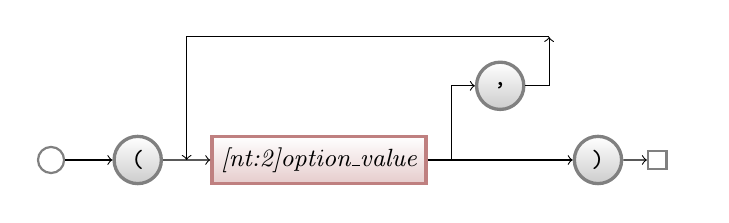
\begin{tikzpicture}
  \matrix[column sep=\ruleMatrixColumnSeparation, row sep=\ruleMatrixRowSeparation] {
    & & & & & & & \node (p2-7) [point] {}; & \\
    & & & & & & \node (p1-6) [terminal] {,}; & \\
    \node (P0start) [firstPoint] {}; & & \node (p0-2) [terminal] {(}; & \node (p0-3) [point] {}; & \node (p0-4) [nonterminal] {\nonTerminalSymbol{option\_value}{2}}; & \node (p0-5) [point] {}; & & & \node (p0-8) [terminal] {)}; & \node (p0-9) [lastPoint] {}; & \\
  };
  \draw[->] (P0start) -- (p0-2) ;
  \draw[->] (p0-2) -- (p0-4) ;
  \draw[->] (p0-5) |- (p1-6) ;
  \draw[->] (p2-7) -| (p0-3) ;
  \draw[->] (p1-6) -| (p2-7) ;
  \draw[->] (p0-4) -- (p0-8) ;
  \draw[->] (p0-8) -- (p0-9) ;
\end{tikzpicture}

\nonTerminalSection{option\_item}{1}

\ruleSubsection{options\_parser}{options\_parser}{39}

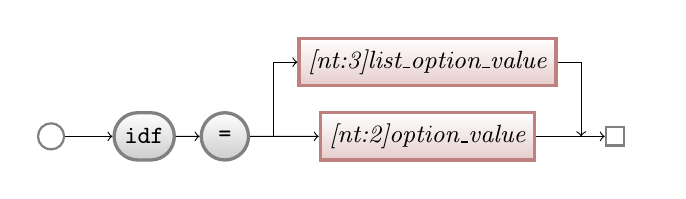
\begin{tikzpicture}
  \matrix[column sep=\ruleMatrixColumnSeparation, row sep=\ruleMatrixRowSeparation] {
    & & & & & \node (p1-5) [nonterminal] {\nonTerminalSymbol{list\_option\_value}{3}}; & \\
    \node (P0start) [firstPoint] {}; & & \node (p0-2) [terminal] {idf}; & \node (p0-3) [terminal] {=}; & \node (p0-4) [point] {}; & \node (p0-5) [nonterminal] {\nonTerminalSymbol{option\_value}{2}}; & \node (p0-6) [point] {}; & \node (p0-7) [lastPoint] {}; & \\
  };
  \draw[->] (P0start) -- (p0-2) ;
  \draw[->] (p0-2) -- (p0-3) ;
  \draw[->] (p0-3) -- (p0-5) ;
  \draw[->] (p0-4) |- (p1-5) ;
  \draw (p0-5) -- (p0-6) ;
  \draw[->] (p1-5) -| (p0-6) ;
  \draw[->] (p0-6) -- (p0-7) ;
\end{tikzpicture}

\nonTerminalSection{option\_parser\_start}{0}

\ruleSubsection{options\_parser}{options\_parser}{29}

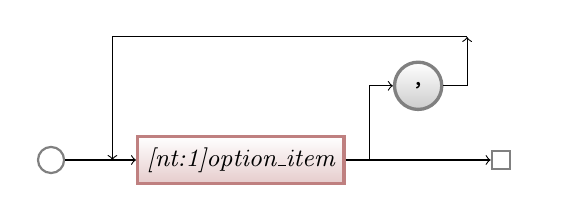
\begin{tikzpicture}
  \matrix[column sep=\ruleMatrixColumnSeparation, row sep=\ruleMatrixRowSeparation] {
    & & & & & & \node (p2-6) [point] {}; & \\
    & & & & & \node (p1-5) [terminal] {,}; & \\
    \node (P0start) [firstPoint] {}; & & \node (p0-2) [point] {}; & \node (p0-3) [nonterminal] {\nonTerminalSymbol{option\_item}{1}}; & \node (p0-4) [point] {}; & & & \node (p0-7) [lastPoint] {}; & \\
  };
  \draw[->] (P0start) -- (p0-3) ;
  \draw[->] (p0-4) |- (p1-5) ;
  \draw[->] (p2-6) -| (p0-2) ;
  \draw[->] (p1-5) -| (p2-6) ;
  \draw[->] (p0-3) -- (p0-7) ;
\end{tikzpicture}

\nonTerminalSection{option\_value}{2}

\ruleSubsection{options\_parser}{options\_parser}{53}

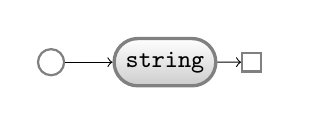
\begin{tikzpicture}
  \matrix[column sep=\ruleMatrixColumnSeparation, row sep=\ruleMatrixRowSeparation] {
    \node (P0start) [firstPoint] {}; & & \node (p0-2) [terminal] {string}; & \node (p0-3) [lastPoint] {}; & \\
  };
  \draw[->] (P0start) -- (p0-2) ;
  \draw[->] (p0-2) -- (p0-3) ;
\end{tikzpicture}

\ruleSubsection{options\_parser}{options\_parser}{60}

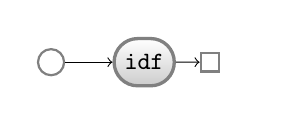
\begin{tikzpicture}
  \matrix[column sep=\ruleMatrixColumnSeparation, row sep=\ruleMatrixRowSeparation] {
    \node (P0start) [firstPoint] {}; & & \node (p0-2) [terminal] {idf}; & \node (p0-3) [lastPoint] {}; & \\
  };
  \draw[->] (P0start) -- (p0-2) ;
  \draw[->] (p0-2) -- (p0-3) ;
\end{tikzpicture}

\ruleSubsection{options\_parser}{options\_parser}{67}

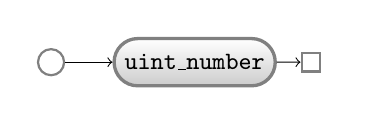
\begin{tikzpicture}
  \matrix[column sep=\ruleMatrixColumnSeparation, row sep=\ruleMatrixRowSeparation] {
    \node (P0start) [firstPoint] {}; & & \node (p0-2) [terminal] {uint\_number}; & \node (p0-3) [lastPoint] {}; & \\
  };
  \draw[->] (P0start) -- (p0-2) ;
  \draw[->] (p0-2) -- (p0-3) ;
\end{tikzpicture}

\ruleSubsection{options\_parser}{options\_parser}{74}

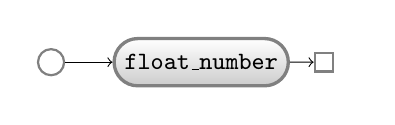
\begin{tikzpicture}
  \matrix[column sep=\ruleMatrixColumnSeparation, row sep=\ruleMatrixRowSeparation] {
    \node (P0start) [firstPoint] {}; & & \node (p0-2) [terminal] {float\_number}; & \node (p0-3) [lastPoint] {}; & \\
  };
  \draw[->] (P0start) -- (p0-2) ;
  \draw[->] (p0-2) -- (p0-3) ;
\end{tikzpicture}

\ruleSubsection{options\_parser}{options\_parser}{81}

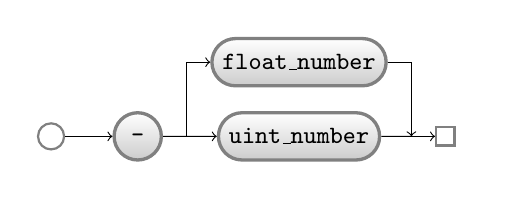
\begin{tikzpicture}
  \matrix[column sep=\ruleMatrixColumnSeparation, row sep=\ruleMatrixRowSeparation] {
    & & & & \node (p1-4) [terminal] {float\_number}; & \\
    \node (P0start) [firstPoint] {}; & & \node (p0-2) [terminal] {-}; & \node (p0-3) [point] {}; & \node (p0-4) [terminal] {uint\_number}; & \node (p0-5) [point] {}; & \node (p0-6) [lastPoint] {}; & \\
  };
  \draw[->] (P0start) -- (p0-2) ;
  \draw[->] (p0-2) -- (p0-4) ;
  \draw[->] (p0-3) |- (p1-4) ;
  \draw (p0-4) -- (p0-5) ;
  \draw[->] (p1-4) -| (p0-5) ;
  \draw[->] (p0-5) -- (p0-6) ;
\end{tikzpicture}



\end{document}
